\documentclass[11pt]{article}

\usepackage{fullpage}
\parindent=0in


%------------------------------------------------------------------
% PROBLEM, PART, AND POINT COUNTING...

% Create the problem number counter.  Initialize to zero.
\newcounter{problemnum}

% Specify that problems should be labeled with arabic numerals.
\renewcommand{\theproblemnum}{\arabic{problemnum}}


% Create the part-within-a-problem counter, "within" the problem counter.
% This counter resets to zero automatically every time the PROBLEMNUM counter
% is incremented.
\newcounter{partnum}[problemnum]

% Specify that parts should be labeled with lowercase letters.
\renewcommand{\thepartnum}{\alph{partnum}}

% Make a counter to keep track of total points assigned to problems...
\newcounter{totalpoints}

% Make counters to keep track of points for parts...
\newcounter{curprobpts}		% Points assigned for the problem as a whole.
\newcounter{totalparts}		% Total points assigned to the various parts.

% Make a counter to keep track of the number of points on each page...
\newcounter{pagepoints}
% This counter is reset each time a page is printed.

% This "program" keeps track of how many points appear on each page, so that
% the total can be printed on the page itself.  Points are added to the total
% for a page when the PART (not the problem) they are assigned to is specified.
% When a problem without parts appears, the PAGEPOINTS are incremented directly
% from the problem as a whole (CURPROBPTS).


%---------------------------------------------------------------------------


% The \problem environment first checks the information about the previous
% problem.  If no parts appeared (or if they were all assigned zero points,
% then it increments TOTALPOINTS directly from CURPROBPTS, the points assigned
% to the last problem as a whole.  If the last problem did contain parts, it
% checks to make sure that their point values total up to the correct sum.
% It then puts the problem number on the page, along with the points assigned
% to it.

\newenvironment{problem}[1]{
% STATEMENTS TO BE EXECUTED WHEN A NEW PROBLEM IS BEGUN:
%
% Increment the problem number counter, and set the current \ref value to that
% number.
\refstepcounter{problemnum}
%
% Add some vspace to separate from the last problem.
\vspace{0.15in} \par
%
\setcounter{curprobpts}{#1} \setcounter{totalparts}{0}	% Reset counters.
%
% Now put in the "announcement" on the page.
{\Large \bf \theproblemnum. \normalsize ({\it \arabic{curprobpts} point\null\ifnum \value{curprobpts} = 1\else s\fi}\/)}
}{
% STATEMENTS TO BE EXECUTED WHEN AN OLD PROBLEM IS ENDED:
%
% If no parts to problem, then increment TOTALPOINTS and PAGEPOINTS for the
% entire problem at once.
\ifnum \value{totalparts} = 0
	\addtocounter{totalpoints}{\value{curprobpts}}	% Add pts to total.
	\addtocounter{pagepoints}{\value{curprobpts}}	% Add pts to page total.
%
% If there were parts for the problem, then check to make sure they total up
% to the same number of points that the problem is worth. Issue a warning
% if not.
\else \ifnum \value{totalparts} = \value{curprobpts}
	\else \typeout{}
	\typeout{!!!!!!!   POINT ACCOUNTING ERROR   !!!!!!!!}
	\typeout{PROBLEM [\theproblemnum] WAS ALLOCATED \arabic{curprobpts} POINTS,}
	\typeout{BUT CONTAINS PARTS TOTALLING \arabic{totalparts} POINTS!}
	\typeout{}
	\fi
\fi
}


%---------------------------------------------------------------------------


% The \newpart command increments the part counter and displays an appropriate
% lowercase letter to mark the part.  It adds points to the point counter
% immediately.  If 0 points are specified, no point announcement is made.
% Otherwise, the announcement is in scriptsize italics.

\newcommand{\newpart}[1]
{
\refstepcounter{partnum}	% Set the current \ref value to the part number.
%\hspace{0.25in}		% Indent the part by a quarter inch.
%
% If points are to be printed for this problem (signaled by point value > 0),
% then put them in in scriptsize italics.
\ifnum #1 > 0
	\makebox[0.25in][l]{{\bf \thepartnum.} {\bf ({\it #1 pt\ifnum #1 = 1\else s\fi\/}) \,\,}}
\else
	\makebox[0.25in][l]{({\bf \thepartnum})}
\fi
%
\hspace{0.1in}		% Lead the material away from the part "number".
%
\addtocounter{totalparts}{#1}	% Add points to totalparts for this problem.
\addtocounter{pagepoints}{#1}	% Add points to total for this page.
\addtocounter{totalpoints}{#1}	% Add points to total for entire test.
}


%---------------------------------------------------------------------------



% Just in case you want to skip some numbers in your test...

\newcommand{\skipproblem}[1]{\addtocounter{problemnum}{#1}}



%---------------------------------------------------------------------------


% The \showpoints command simply gives a count of the total points read in up to
% the location at which the command is placed.  Typically, one places one
% \showpoints command at the end of the latex file, just prior to the
% \end{document} command.  It can appear elsewhere, however.

\newcommand{\showpoints}
{
\typeout{}
\typeout{====> A TOTAL OF \arabic{totalpoints} POINTS WERE READ.}
\typeout{}
}


%---------------------------------------------------------------------------



\usepackage{graphicx}
\usepackage[english]{babel}
\usepackage[latin1]{inputenc}
\usepackage{times}
\usepackage[T1]{fontenc}
\usepackage{amsmath}
\usepackage{amssymb}
\usepackage{hyperref}
\usepackage{color}
\usepackage{bbm}
\usepackage{algorithm}
\usepackage{algpseudocode}

\begin{document}

{\centering
  \rule{6.3in}{2pt}
  \vspace{1em}
  {\Large
    CS589: Machine Learning - Fall 2018\\
    Homework 3: Kernels\\
  }
  \vspace{1em}
  Assigned: November $9^{th}$, 2018 Due: November $26^{th}$, 2018\\
  \vspace{0.1em}
  \rule{6.3in}{1.5pt}
}
\vspace{1pc}

\textbf{Getting Started:} In this assignment, you will train and evaluate different kernels for both classification and regression on three datasets. Please install Python 3.6 via Anaconda on your personal machine. For this homework you will only be using numpy, scipy, sklearn and matplotlib packages. Download the homework file HW03.zip via Moodle. Unzipping this folder will create the directory structure shown below,
\begin{verbatim}
HW03
--- HW03.pdf
--- Data
    |--Synthetic
    |--CreditCard
    |--Tumor
--- Submission
    |--Code
    |--Figures
    |--Predictions
       |--CreditCard
       |--Tumor
\end{verbatim}
The data files for each data set are in `Data' directory respectively. You will write your code under the Submission/Code directory. Make sure to put the deliverables (explained below) into the respective directories.

\vspace{5mm}
\textbf{Deliverables:} This assignment has three types of deliverables:
\begin{itemize}
\item \textbf{Report:} The solution report will give your answers to the homework questions (listed below). You  may use as many pages as you wish, so long as you assign your pages appropriately on Gradescope.  You can use any software to create your report, but your report must be submitted in PDF format. 

\item \textbf{Code:} The second deliverable is the code that you wrote to answer the questions, which will involve implementing kernel methods. Your code must be Python 3.6 (no iPython notebooks or other formats). You may create any additional source files to structure your code. However, you should aim to write your code so that it is possible to re-produce all of your experimental results exactly by running \textit{python run\_me.py} file from the Submissions/Code directory.

\item \textbf{Kaggle Submissions:} We will use Kaggle, a machine learning competition service, to evaluate the performance of your regression models. You will need to register on Kaggle using a *.edu email address to submit to Kaggle (you can use any user name you like). There is also a Moodle quiz for you to enter your Kaggle username so that we can map your results automatically. You will generate test prediction files, save them in Kaggle format (helper code provided called \textit{Code/kaggle.py}) and upload them to Kaggle for scoring. Your scores will be shown on the Kaggle leaderboard.
The Kaggle links for each data set are given under respective questions.

\end{itemize}
\vspace{1em}

\textbf{Submitting Deliverables:}
When you complete the assignment, you will upload your report and your code using the Gradescope.com service. Place your final code in Submission/Code, and the Kaggle prediction files for your best-performing submission only for each data set in Submission/Predictions/<Data Set>/best.csv. Naming your files something other than best.csv breaks our grading scripts. Please try to name them best.cav. If you used Python to generate report figures, place them in Submission/Figures. Finally, create a zip file of your submission directory, Submission.zip (NO rar, tar or other formats). Upload this single zip file on Gradescope as your solution to the 'HW02-Kernel-Programming' assignment. Gradescope will run checks to determine if your submission contains the required files in the correct locations. Finally, upload your pdf report to the 'HW03-Kernel-Report' assignment. When you upload your report please make sure to select the correct pages for each question respectively. Failure to select the correct pages will result in point deductions. The submission time for your assignment is considered to be the later of the submission timestamps of your code, report and Kaggle submissions.\\

\textbf{Academic Honesty Statement:} Copying solutions from external sources (books, internet, etc.) or other students is considered cheating. Sharing your solutions with other students is also considered cheating. Posting your code to public repositories like GitHub, stackoverflow is also considered cheating. Any detected cheating will result in a grade of -100\% on the assignment for all students involved, and potentially a grade of F in the course.\\

\textbf{Task:} 
In this homework you will experimenting with kernel methods for regression and classification problems using kernel ridge regression and support vector machine (SVM).
\begin{enumerate}
\item \textbf{Kernel Ridge Regression:} This is a kernel regression method. Let $\{x_i, y_i\}$ be the set of inputs, the problem consists on finding the $w$ that minimizes,
\begin{align}
\sum_{i} (x_i \cdot w - y_i) ^ 2 + \lambda \Vert w \Vert_2^2
\end{align}
where, the first term corresponds to the squared loss in the estimation, and the second is a regularization term. As seen during the lectures, one can apply a transformation to the samples (which increases their dimensionality) and perform the linear regression in this new higher dimensional space, which will correspond to a non-linear regression in the original space. An extremely important note regarding this is that, in order to estimate the value corresponding to a new sample $x_{new}$, only the inner product $x_{new} \cdot x_i$ is necessary. Thus, the kernel trick is applicable.\\
\item \textbf{SVM:} This is a classification method that can assign classes to new samples using only the inner product between the new samples and the samples in the training data. This allows us to use several different kernels, which makes SVM an extremely powerful classification method.\\
\end{enumerate}

\textbf{Data:} You will work with three datasets,

\begin{itemize}
\item \textbf{Synthetic:} Use this dataset to check equivalence between basis expansion and the use of kernels in regression settings. You are provided four files: data\_train.txt, label\_train.txt, data\_test.txt and label\_test.txt.
\item \textbf{CreditCard:} This dataset has eight attributes and two outputs, all real numbers. We treat this is as a regression problem. The attributes correspond to credit card activity of individuals, and the outputs are two measure of risk as established by experts in the bank. You are provided three files: data\_train.txt, label\_train.txt and data\_test.txt.
\item \textbf{Tumor:} This dataset has nine attributes and a binary output. We treat this as a classification problem. The attributes are different measurements obtained from a medical imaging, and the output corresponds to the presence/absence of tumor. You are provided three files: data\_train.txt, label\_train.txt and data\_test.txt.
\end{itemize}

Code to load datasets is provided in \textit{run\_me.py}. Below is a summary of the datasets, allowed python functions per dataset and performance metric to report in your HW03 pdf report which matches with Kaggle's performance reporting.

\begin{table}[H]
\centering
\begin{tabular}{|c|c|c|c|}\hline
\textbf{Dataset} & \textbf{Python functions} & \textbf{Use} & \textbf{Metric} \\\hline
Synthetic & sklearn.kernel\_ridge.* & Not allowed & Mean squared error \\
          & Inbuilt Basis expansions & Not allowed & (regression) \\
          & sklearn.linear\_model.Ridge & Allowed & \\\hline
Credit Card & sklearn.kernel\_ridge.* & Allowed & Mean squared error \\
	    & sklearn.model\_selection.* & Allowed & (regression) \\\hline
Tumor & sklearn.svm.* & Allowed & Accuracy \\
      & sklearn.model\_selection.* & Allowed & (classification)\\\hline
\end{tabular}
\end{table}

This homework will be scored out of 115 points, with a maximum possible score of 125 via extra credit points.  Note this is different from the previous homework in that it is possible to score over 100\%.\\

\textbf{Questions:}
\begin{problem}{20} \textbf{Quadratic Kernel:} 
\begin{description}
	\item[(10) a.] Consider the quadratic kernel and quadratic basis expansion given in lecture:
	
	\begin{align*}
	K(x,y) &= (x^Ty)^2\\
	\phi([x_1,x_2]) &= (x_1x_1,x_1x_2,x_2x_1,x_2x_2)
	\end{align*}
	
	 Let $x,y$ be restricted to 2-dimensional vectors.  Show that $K(x,y) = \phi(x)^T \phi(y)$.
	 
	 \item[(10) b.] Let $\phi(x)$ be defined for arbitrary $n$-length vectors:
	 
	 $$\phi(x) = \{x_ix_j \mid \forall i = 1...n, \forall j = 1....n\}$$
	 
	 Show that $K(x,y) = \phi(x)^T \phi(y)$ for arbitrary $n$-length vectors.
\end{description}



\end{problem}


\begin{problem}{75} \textbf{Kernel Ridge Regression:}

\begin{description}
\item[(11) a.] Kernel Ridge Regression was introduced above. The goal is to find $w$ that minimizes 
\begin{align}
\sum_{i} (x_i \cdot w - y_i) ^ 2 + \lambda \Vert w \Vert_2^2
\end{align}
Once the optimal $w$, $w^*$, is found, it can be used to estimate the value of new samples as $y_{est} = w^* \cdot x_{new}$. Show that, without using basis expansion nor kernels, the optimal $w$ is, 
\begin{align}
w^* = \big ( \sum_i x_i \, x_i^T + \lambda \, I \big ) ^ {-1} \sum_i x_i \, y_i
\end{align}
\item[(4) b.] Show the expression of $w^*$ for the case in which a basis expansion $x \rightarrow \Phi(x)$ is used.
\item[(10) c.] As mentioned above, for this type of regression the kernel trick is applicable. This means that it is not necessary to know the transformation $\Phi$; having an expression for $\Phi(x_1) \cdot \Phi(x_2)$ (inner product of two samples in the new space) suffices. Given a new sample $x_{new}$, derive an expression for $y_{new}$ that depends only on inner products between samples.

\item[(30) d.] In this exercise you will perform Kernel Ridge Regression using the synthetic dataset with samples $x_i \in \mathbb{R}$ and labels $y_i \in \mathbb{R}$. The training data is in \textit{data\_train.txt, label\_train.txt}, and the testing data is in \textit{data\_test.txt, label\_test.txt}. The training data is shown in Fig. \ref{fig:data1d}.

\begin{figure}[H]
  \centering
  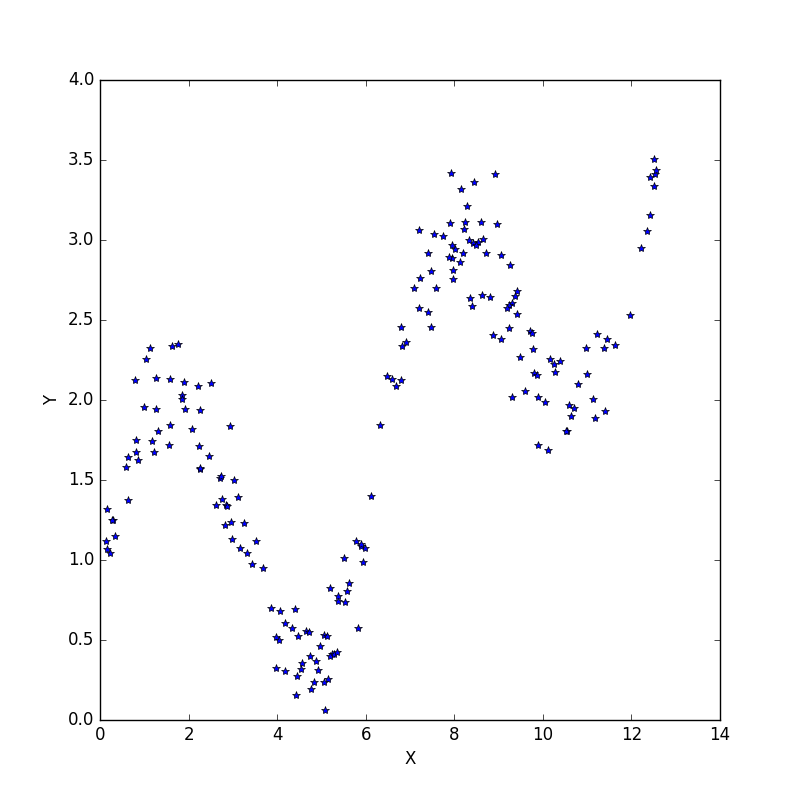
\includegraphics[width=0.45\textwidth]{train.png}
  \caption{Data}
  \label{fig:data1d}
\end{figure}

We would like you to implement kernel ridge regression from scratch. What this means is the following:

\begin{itemize}
	\item  \textbf{only} for this question when it reads `Kernel ridge regression scratch (KRRS)' we expect you to use your \textbf{own handwritten} kernel ridge regression
	\item when it reads `Basis Expansion + ridge regression (BERR)' we expect you to compute the basis expansion again by hand, but you are free to use these expanded basis feature vectors with sklearn's ridge regression or your own implementation of ridge regression.
	\item To be clear, you are \textbf{NOT allowed} to use `sklearn.kernel\_ridge.KernelRidge' or any of its variants for KRRS and built in basis expansion functions for BERR.
\end{itemize}

We would like you to compare the performance of the two approaches on the synthetic dataset to better understand kernel methods. As mentioned in the class, the implementation using a kernel $k(x_i, x_j) = \Phi(x_i) \cdot \Phi(x_j)$ should return the same results as the implementation using the basis expansion $\Phi$ followed by ridge regression. You will use the following parameters for KRRS/BERRs (with $\lambda = 0.1$):\\

\textbf{Polynomial order i:} (for $i \in \{1,2,4,6\}$)\\
\begin{enumerate}
\item Kernel ridge regression scratch (KRRS):
\begin{align}
k(x_1, x_2) = (1 + x_1 \cdot x_2) ^ i
\end{align}
\item Basis expansion + ridge regression (BERR):
\begin{align}
\Phi(x) = [1, x^1, x^2, ..., x^i]
\end{align}
\end{enumerate}
\textbf{Trigonometric order i:} (for $i \in \{3, 5, 10\}$)\\
\begin{enumerate}
\item Kernel ridge regression scratch (KRRS):
\begin{align}
k(x_1, x_2) = 1 + \sum_{k = 1}^{i} (\sin(k\,\delta \, x_1) \cdot \sin(k\,\delta \, x_2) + \cos(k\,\delta \, x_1) \cdot \cos(k\,\delta \, x_2) )
\end{align}
\item Basis expansion + ridge regression (BERR):
\begin{align}
\Phi(x) = [1, \sin(\delta \, x), \cos(\delta \, x), \sin(2\delta \, x), \cos(2\delta \, x), ..., \sin(i \,\delta \, x), \cos(i \,\delta \, x)]
\end{align}
\end{enumerate}
With $\delta = 0.5$.\\

\begin{description}
\item[1.] Train your models using the train data and predict the outputs for the test data. Visually inspect the quality of predictions by plotting the predicted test labels on top of the original test labels as a function of test data. Make these plots corresponding to polynomial kernels of degree 2 and 6, and trigonometric kernels of degree 5 and 10 only. A sample plot is provided in Figure \ref{fig:py_plot1d}. In each plot include the test samples as blue `*' and plot the predictions made on the test set as red circles. Make sure to label the axis, and include a title for each graph with implementation, kernel, degree and lambda used. Arrange your plots as a 4 $\times$ 2 grid (i.e. four rows and 2 columns; see \textit{matplotlib.pyplot.subplot}) where the four rows correspond to the kernels and the two columns correspond to the two implementations. Write in at most three sentences what your observations are about these eight plots.

\begin{figure}[H]
  \centering
  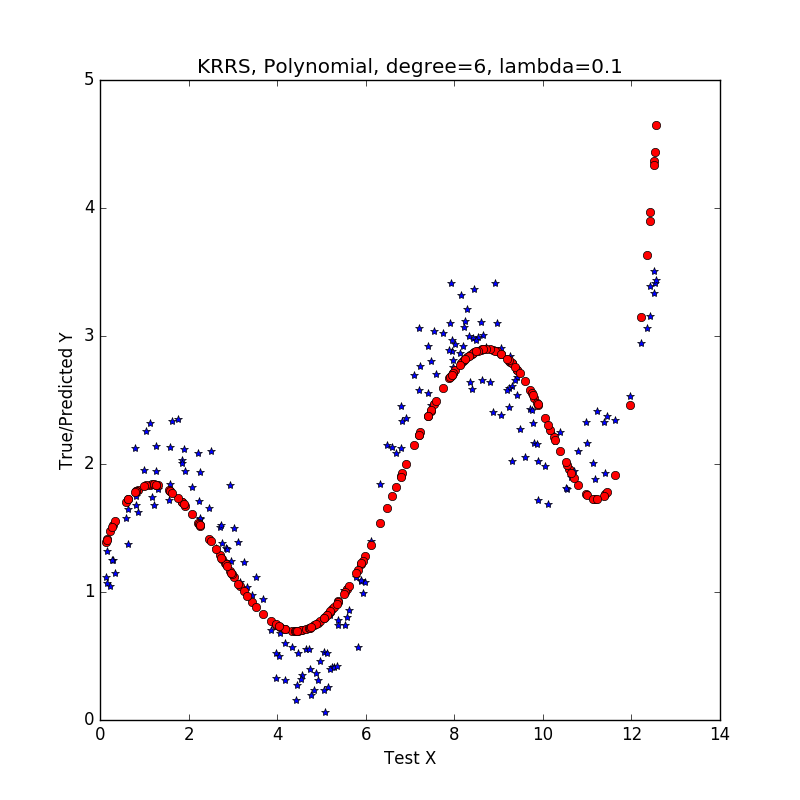
\includegraphics[width=0.5\textwidth]{py_plot1d.png}
  \caption{Test samples are plotted in blue `*' and predicted test labels are plotted in red `o'}
  \label{fig:py_plot1d}
\end{figure}

\item[2.] For each of the kernels/basis expansions mentioned above, show the mean squared error over the \textbf{test set} using a table like the one below (please make the table exactly as shown below to make grading more efficient),

\begin{table}[H]
\centering
\begin{tabular}{|l|c|c|}
\hline
                & Kernel $k(x_1, x_2)$ & Basis Expansion $\Phi(x)$ \\ \hline
Polynomial degree 1   &                      &                           \\ \hline
Polynomial degree 2   &                      &                           \\ \hline
Polynomial degree 4   &                      &                           \\ \hline
Polynomial degree 6   &                      &                           \\ \hline
Trignometric degree 3  &                      &                           \\ \hline
Trignometric degree 5  &                      &                           \\ \hline
Trignometric degree 10 &                      &                           \\ \hline
\end{tabular}
\end{table}
where in each empty box you need to write the mean squared error obtained via KRRS or BERR.

\end{description}

\item[(20) e.] In this exercise you will perform Kernel Ridge Regression using the credit card activity dataset.
For this question you are allowed to (and encouraged) use sklearn's implementation of Kernel Ridge Regression.
You will train several kernels (radial basis functions, polynomial degree 3, linear) with parameters - $\alpha \in \{1, 0.0001\}$ and $\gamma \in \{\text{default}, 1, 0.001\}$ (the default parameter is when you don't specify any $\gamma$).
In total you will need to train and test 14 models (the $\gamma$ parameter does not have any effect on linear kernels).
For each kernel, pick your choice of model selection method to estimate the out of sample mean squared error.
Report the results in a table format as shown below (please make the table exactly as shown below to make grading more efficient),

\begin{table}[H]
\centering
\begin{tabular}{|l|c|c|c|}
\hline
                                    & RBF & Poly. degree 3 & Linear \\\hline
$\alpha = 1$, $\gamma = def$        &     &       &        \\\hline
$\alpha = 1$, $\gamma = 1$          &     &       & ---    \\\hline
$\alpha = 1$, $\gamma = 0.001$      &     &       & ---    \\\hline
$\alpha = 0.0001$, $\gamma = def$   &     &       &        \\\hline
$\alpha = 0.0001$, $\gamma = 1$     &     &       & ---    \\\hline
$\alpha = 0.0001$, $\gamma = 0.001$ &     &       & ---    \\\hline
\end{tabular}
\end{table} 

Choose the model with lowest estimated out of sample error, train it using the full training set, make predictions on the test set, kagglize your outputs (helper code given in \textit{Code/kaggle.py}) and finally upload your predictions to Kaggle.
The Kaggle link to this question is\\
\url{https://www.kaggle.com/t/1110f6dd270b4a96835dac15646eafa4}.\\
Report back the mean squared error that you obtained on the public leader board as well as your Kaggle display name so that we can match your results with your rank on the leaderboard. Make sure to clearly indicate which model provided the best results as well as your choice of model selection method.
Finally, consider the results that you obtained on the train set (via model selection) as well as your test results.
Compare the two  and draw some conclusions on your chosen kernel, specific parameter settings and its relation to the dataset itself.

\end{description}
\end{problem}




\begin{problem}{25}\textbf{SVM:}
\begin{description}
\item[(25) a.] For this question you will use perform classification using a SVM on the tumor dataset.
For this question you are allowed to (and encouraged) use sklearn's implementation of SVM.
You will train an SVM classifier using the kernels shown in the below table, and complete the table using estimates of the out of sample accuracy (NOT error but classification accuracy) obtained using your choice of model selection method.





\begin{table}[H]
\centering
\begin{tabular}{|l|c|c|c|c|}
\hline
                                    & RBF & Poly. degree 3 & Poly. degree 5 & Linear \\\hline
$C = 1$, $\gamma = 1$        &     &  &    &        \\\hline
$C = 1$, $\gamma = 0.01$          &     &  &    &  ---      \\\hline
$C = 1$, $\gamma = 0.001$      &     &  &    &  ---      \\\hline
$C = 0.01$, $\gamma = 1$   &     &    &  &        \\\hline
$C = 0.01$, $\gamma = 0.01$     &     &    &  &  ---      \\\hline
$C = 0.01$, $\gamma = 0.001$ &     &    &  &  ---      \\\hline
$C = 0.0001$, $\gamma = 1$ &     &  &    &        \\\hline
$C = 0.0001$, $\gamma = 0.01$ &     &  &    &    ---    \\\hline
$C = 0.0001$, $\gamma = 0.001$ &     &  &    &   ---     \\\hline
\end{tabular}
\end{table} 

Again here the $\gamma$ parameter does not have any effect on linear kernels.
\vspace{2mm}

Choose the model with highest estimated out of sample accuracy, train it using the full training set, make predictions on the test set, kagglize your outputs (helper code given in \textit{Code/kaggle.py}) and finally upload your predictions to Kaggle.
The Kaggle link to this question is\\
\url{https://www.kaggle.com/t/eb79c33955334af09a4c7970794d01d4}.\\
Report back the classification accuracy that you obtained on the public leader board as well as your Kaggle display name so that we can match your results with your rank on the leaderboard. Make sure to clearly indicate which model provided the best results and your choice of model selection method.
Finally, consider the results that you obtained on the train set (via model selection) as well as your test results.
Compare the two and draw some conclusions on your chosen kernel, specific parameter settings and its relation to the dataset itself.


\end{description}
\end{problem}

\begin{problem}{0}\textbf{Moodle Quiz}
	Did you submit your Kaggle username on the Moodle quiz (Y/N)?  Please make sure you use the same username across all Kaggle submission on this homework.\\
	See the following link -  \url{https://moodle.umass.edu/mod/questionnaire/view.php?id=1719866}?
\end{problem}
\vspace{3mm}

\textbf{Extra Credit: These questions are deliberately open-ended, leaving you more space for creativity.
As a result, you will need to carefully describe exactly what you did for each question.
Also, note that these questions carry small point values. To maximize your score with limited time, you should make sure the above questions are done thoroughly and ignore these. We will be very stingy in giving credit for these questions -- do them only for the glory, and only at your own risk!}

\begin{problem}{5} \textbf{Extra credit:} For the credit card dataset perform regression with your choice of kernels (you are free to even create your own kernels). Experiment with different parameter ranges and/or model selection methods with a single goal of improving performance on the held out test set. For this extra credit question the kaggle URL to submit your predictions is\\
\url{https://www.kaggle.com/t/f79f4b4c7f4441be81d8d46f2230afe8}.\\
Make sure to clearly describe your approach and list your performance on the public leaderboard. To avoid any confusion make sure to write the outputs to Predictions/CreditCard/best\_extra\_credit.csv. Note that your grades will be dependent on your ranking in the private leaderboard.
\end{problem}

\begin{problem}{5} \textbf{Extra credit:} For the tumor dataset perform classification with your choice of kernels. Experiment with different parameter ranges and/or model selection methods with a single goal of improving performance on the held out test set. For this extra credit question the kaggle URL to submit your predictions is\\
\url{https://www.kaggle.com/t/f174cd4ecda7425c978e936dfc37e9e5}.\\
Make sure to clearly describe your approach and list your performance on the public leaderboard. To avoid any confusion make sure to write the outputs to Predictions/Tumor/best\_extra\_credit.csv. Note that your grades will be dependent on your ranking in the private leaderboard.
\end{problem}



\showpoints
\end{document}
